\documentclass[11pt,a4paper,oneside,english]{amsart}

\usepackage{showlabels}
\usepackage[boxed]{algorithm2e}
\usepackage{amsaddr}
\usepackage{babel}
\usepackage{amssymb}
\usepackage{bm}
\usepackage{booktabs}
\usepackage{commath}
\usepackage{colortbl}
\usepackage{dsfont}
\usepackage{enumerate}
\usepackage{esint}
\usepackage[left=0.09\paperwidth, right=0.15\paperwidth, bottom=0.12\paperheight]{geometry}
\usepackage{graphicx}
\usepackage[displaymath, mathlines]{lineno}
\usepackage{mathtools}
\usepackage{mathrsfs}
\usepackage{multirow,bigdelim}
\usepackage{url}
\usepackage{pdflscape}
\usepackage{rotating}
%\usepackage[outer]{showlabels}
\usepackage[color=white,linecolor=black, textwidth=0.12\paperwidth]{todonotes}
%\setlength{\parindent}{0pt}
\usepackage{wrapfig}

\numberwithin{equation}{section}
\newtheorem{theorem}{Theorem}
\numberwithin{theorem}{section}
\newtheorem{assum}[theorem]{Assumption}
\newtheorem{lemma}[theorem]{Lemma}
\newtheorem{corol}[theorem]{Corollary}
\newtheorem{prop}[theorem]{Proposition}
\theoremstyle{definition}
\newtheorem{remark}[theorem]{Remark}
\newtheorem{example}[theorem]{Example}

\usepackage{color}
\newcommand{\R}{\mathbb{R}}
\newcommand{\N}{\mathbb{N}}
\newcommand{\Z}{\mathbb{Z}}
\providecommand\C{}
\renewcommand{\C}{\mathbb{C}}
\newcommand{\A}{\mathcal{A}}
\newcommand{\Q}{\mathbb{Q}}
\newcommand{\E}{\mathcal{E}}
\newcommand{\F}{\mathbb{F}}
\newcommand{\D}{\mathcal{D}}
\newcommand{\K}{\mathcal{K}}
\renewcommand{\H}{\mathcal{H}}
\newcommand{\B}{\mathcal{B}}
\newcommand{\M}{\mathcal{M}}
\newcommand{\bbD}{\mathbb{D}}
\newcommand{\f}{\varphi}
\newcommand{\e}{\varepsilon}
\newcommand{\eps}{\varepsilon}
\renewcommand{\a}{\alpha}
\renewcommand{\b}{\beta}
\newcommand{\z}{\zeta}
\renewcommand{\O}{\Omega}
\renewcommand{\P}{\mathbb P}
\newcommand{\intRn}{\int_{\R^n}}
\newcommand{\sumi}{\sum_{i=1}^n}
\newcommand{\sumij}{\sum_{i,j=1}^n}
\renewcommand{\d}{\delta}
\newcommand{\p}{\partial}
\DeclareMathOperator{\osc}{osc}
\DeclareMathOperator{\supp}{supp}
\DeclareMathOperator{\vol}{vol}
\DeclareMathOperator{\gen}{gen}
\DeclareMathOperator{\cat}{Cat}
\DeclareMathOperator{\Cat}{Cat}
\DeclareMathOperator{\Div}{div}
\DeclareMathOperator{\blockdiag}{blockdiag}
\renewcommand{\div}{\Div}
\DeclareMathOperator{\spann}{span}
\DeclareMathOperator{\diam}{diam}
\DeclareMathOperator{\dist}{dist}
\newcommand{\la}{\langle}
\newcommand{\ra}{\rangle}
\usepackage{stmaryrd}
\newcommand{\jump}[1]{\left\llbracket #1 \right\rrbracket}
\newcommand{\rhu}{\rightharpoonup}
\newcommand{\T}{\mathcal{T}}
\newcommand{\V}{\mathcal{V}}
\DeclareMathOperator*{\dof}{\#\!DoF}
\DeclareMathOperator*{\argmin}{arg\,min}
\DeclareMathOperator*{\Id}{Id}
\definecolor{airforceblue}{rgb}{0.36, 0.54, 0.66}
\definecolor{ao(english)}{rgb}{0.0, 0.5, 0.0}
\providecommand\note{}
\newcommand{\new}[1]{{\color{ao(english)} #1}}
\renewcommand{\L}{\mathcal L}
\newcommand{\Y}{\mathcal Y}
\newcommand{\Lto}{{L_2(\Omega)}}
\newcommand{\bbT}{\mathbb{T}}
\newcommand{\cL}{\mathcal L}
\newcommand{\Lis}{\cL\mathrm{is}}
\newcommand{\udelta}{{\underline{\delta}}}
\newcommand{\jw}[1]{{\color{red}{JW: #1}}}
\newcommand{\rvv}[1]{{\color{teal}{RvV: #1}}}
\DeclareMathOperator*{\ran}{ran}
\SetKwRepeat{Do}{do}{while}%

% Math symbol font matha
\DeclareFontFamily{U}{matha}{\hyphenchar\font45}
\DeclareFontShape{U}{matha}{m}{n}{
      <5> <6> <7> <8> <9> <10> gen * matha
      <10.95> matha10 <12> <14.4> <17.28> <20.74> <24.88> matha12
      }{}
\DeclareSymbolFont{matha}{U}{matha}{m}{n}
\DeclareFontSubstitution{U}{matha}{m}{n}

% Math symbol font mathb
\DeclareFontFamily{U}{mathx}{\hyphenchar\font45}
\DeclareFontShape{U}{mathx}{m}{n}{
      <5> <6> <7> <8> <9> <10>
      <10.95> <12> <14.4> <17.28> <20.74> <24.88>
      mathx10
      }{}
\DeclareSymbolFont{mathx}{U}{mathx}{m}{n}
\DeclareFontSubstitution{U}{mathx}{m}{n}

% Symbol definition
\DeclareMathDelimiter{\vvvert}{0}{matha}{"7E}{mathx}{"17}

\DeclareMathOperator{\ext}{ext}
\DeclareMathOperator{\eff}{eff}
\DeclareMathOperator{\loc}{loc}
\DeclareMathOperator{\irr}{int}
\DeclareMathOperator{\RT}{RT}
\DeclareMathOperator{\meas}{meas}
\newcommand{\bbone}{\mathds{1}}
\newcommand{\bbzero}{\mathds{0}}
\newcommand{\seminorm}[1]{\vvvert #1 \vvvert}
\newcommand{\ltwonorm}[1]{\lVert #1 \rVert}
\newcommand{\hta}{{\check \T_a}}
\newcommand{\hT}{{\check T}}
\newcommand{\he}{{\check e}}
\newcommand{\hE}{{\check \E}}
\newcommand{\dr}{{\tilde r}}
\renewcommand{\emptyset}{{\varnothing}}
\newcommand{\hprime}[1]{H^1_{*, #1}(\hta)}
\newcommand{\laplace}{\mathcal{4}}

\DeclareFontFamily{U}{mathx}{\hyphenchar\font45}
\DeclareFontShape{U}{mathx}{m}{n}{
      <5> <6> <7> <8> <9> <10>
      <10.95> <12> <14.4> <17.28> <20.74> <24.88>
      mathx10
      }{}
\DeclareSymbolFont{mathx}{U}{mathx}{m}{n}
\DeclareFontSubstitution{U}{mathx}{m}{n}
\DeclareMathAccent{\widecheck}{0}{mathx}{"71}
\DeclareMathAccent{\wideparen}{0}{mathx}{"75}
%\linenumbers

\def\cs#1{\texttt{\char`\\#1}}

\title{Space-time adaptivity for parabolic evolution equations}
\author{Rob Stevenson \and Raymond van Veneti\"e \and Jan Westerdiep}
\address{Korteweg-de Vries Institute for Mathematics, University of Amsterdam, \\
P.O. Box 94248, 1090 GE Amsterdam, The Netherlands}
\date{\today}
\subjclass[2010]{}

\thanks{\emph{Funding:} The second and third authors are supported by the Netherlands Organisation for Scientific Research (NWO) under contract.~no.~613.001.652}

\begin{document}
\begin{abstract}
\end{abstract}

\maketitle

\section{Introduction}
\section{Problem statement and solution}
Let $V$ and $H$ be separable Hilbert spaces on a spatial domain $\Omega$ such that
$V \hookrightarrow H$ with dense and compact embedding. Identifying $H$ with its
dual, we obtain the Gelfand triple $V \hookrightarrow H \simeq H' \hookrightarrow V'$.

We use the notation $\la \cdot,\cdot \ra$ to denote both the scalar product
on $H \times H$, and its unique extension by continuity to the duality pairing on
$V' \times V$. Correspondingly, the norm on $H$ will be denoted by $\|\cdot\|$.

Let $T \in (0, \infty)$ be given, and set $I := (0, T)$. We make the following assumption.
\begin{assum}
  \label{assum:a}
  For a.e.~$t$, let $a(t;\cdot,\cdot)$ denote a bilinear form on $V \times V$ that is
  \begin{alignat*}{3}
    t \mapsto a(t; \eta, \zeta) & ~~ \text{is measurable} \quad && (\eta, \zeta \in V), \\
    |a(t;\eta,\zeta)| & \lesssim  \|\eta\|_{V} \|\zeta\|_{V} &&(\eta,\zeta \in V) &\quad&\text{(bounded)}, \\
     a(t;\eta,\eta)   & \gtrsim   \|\eta\|_{V}^2 &&(\eta \in {V}) &&\text{(coercive)}.
  \end{alignat*}
\end{assum}

With $A(t) \in \Lis({V},V')$ being defined by $ (A(t) \eta)(\zeta)=a(t;\eta,\zeta)$,
we are interested in solving the {\em parabolic initial value problem} of finding
$u$ such that
\begin{equation}
  \label{eqn:ibvp}
  \left\{
    \begin{array}{rl}
      \frac{\dif u}{\dif t}(t) +A(t) u(t)&\!\!\!= g(t) \quad(t \in I),\\
      u(0) &\!\!\!= u_0.
    \end{array}
  \right.
\end{equation}

In a simultaneous space-time variational formulation, the parabolic PDE reads as
finding $u$ from a suitable space of functions of time and space such that
\begin{equation}
  \label{eqn:B-var-form}
  (Bw)(v):=\int_I \la \tfrac{\dif w}{\dif t}(t), v(t) \ra + a(t;w(t),v(t)) \dif t = \int_I \la g(t), v(t) \ra =:g(v)
\end{equation}
for all $v$ from another suitable space of functions of time and space.

\begin{theorem}
  \label{thm:varform}
  With $X:=L_2(I;{V}) \cap H^1(I;V')$, $Y:=L_2(I;{V})$, under assumption \ref{assum:a}, we have
  \begin{equation}
    \label{eqn:B-lis}
    \begin{bmatrix} B \\ \gamma_0\end{bmatrix}\in \Lis(X,Y' \times H),
  \end{equation}
  where for $t \in \bar I$, $\gamma_t\colon u \mapsto u(t,\cdot)$ denotes the trace map.
  In other words, given $(g, u_0) \in Y' \times H$, finding $u \in X$ such that
  \begin{equation}
    \label{eqn:B-varform}
    (Bu)(v_1)+\la u(0,\cdot),v_2\ra=g(v_1)+\la u_0,v_2\ra\quad ((v_1,v_2) \in Y \times H),
  \end{equation}
  is a well-posed variational formulation of \eqref{eqn:ibvp}.
\end{theorem}

\subsection{Andreev formulation}
Defining $A, A_s \in \Lis(Y,Y')$, $A_a \in \cL(Y,Y')$, and $\partial_t \in \cL(X,Y')$ by
\[
(Au)(v):=\int_I a(t;u(t),v(t)) \dif t, \quad A_s:=\tfrac12(A+A'), \quad A_a:=\tfrac12(A-A'), \quad \partial_t:=B-A,
\]
an equivalent self-adjoint saddle point formulation of \eqref{eqn:B-varform} was
introduced by Andreev in \cite{Andreev2013} as finding the solution $(\mu,u) \in Y\times X$ of
\[
  \begin{bmatrix} A_s & B\\ B' & -\gamma_0' \gamma_0 \end{bmatrix}
  \begin{bmatrix} \mu \\ u \end{bmatrix}=
  \begin{bmatrix} g \\ -\gamma_0' u_0 \end{bmatrix}.
\]
Thanks to \eqref{eqn:B-lis}, the Schur complement operator $S := B' A_s^{-1} B+\gamma_0'\gamma_0$ is self-adjoint, coercive, and in $\Lis(X, X')$.

\begin{remark}
  For some quantitative estimates to be valid, we assume that $A=A_s$, but we do not expect this to be essential.
\end{remark}
We equip $Y$ and $X$ with the `energy' norms
$$
\|\cdot\|_Y^2:=(A_s\cdot)(\cdot),\quad \|\cdot\|_X^2:=\|\cdot\|_Y^2+\|\partial_t \cdot\|_{Y'}^2+\|\gamma_T \cdot\|^2,
$$
which are equivalent to the canonical norms on $Y$ and $X$.

\begin{lemma}
  \label{lem:energy-norm}
  It holds that $\|\cdot\|_X^2=(S\cdot)(\cdot)$.
\end{lemma}
\begin{proof}
  We find \jw{dit ben ik nog niet nagegaan}
  \[
    \|w\|_X^2=\sup_{0 \neq v_1 \in Y} \frac{(B w)(v_1)}{\|v_1\|_Y^2}+\|\gamma_0 w\|^2
    =\sup_{0 \neq (v_1,v_2) \in Y \times H} \frac{((B w)(v_1)+\la \gamma_0 w,v_2\ra)^2}{\|v_1\|_Y^2+\|v_2\|^2} =(Sw)(w),
  \]
  where the first equality can be found in e.g.~\cite[Thm.~2.1]{Ern2017a}, and,
  when realising that $S$ is also the Schur complement of
  $\begin{bsmallmatrix} A_s & 0 & B\\ 0 & \Id & \gamma_0\\ B' & \gamma_0' & 0\end{bsmallmatrix} \in \cL(Y\times H \times X, Y'\times H'\times X')$, the last one follows from e.g.~\cite[Lemma~2.2]{Kondratyuk2008}.
\end{proof}

Let $(X^\delta)_{\delta \in \Delta}$ be a collection of closed subspaces of $X$.
We define a \emph{partial order} on $\Delta$ by $\delta \preceq \tilde{\delta}$
when $X^\delta \subseteq X^{\tilde{\delta}}$. For $\delta \in \Delta$, let
$u_\delta \in X^\delta$ denote the {\em Galerkin approximation to $u$}, i.e., the solution of
\begin{equation}
(Su_\delta)(v)=f(v) \quad (v \in X^\delta),
  \label{eqn:galerkin}
\end{equation}
being the best approximation to $u$ from $X^\delta$ wrt.~$\|\cdot\|_X$.

\subsection{Discretized problem}
Applying $S$ requires the application of the nonlocal operator $A_s^{-1}$, making it
unsuitable for practical computation. To that end, let $(Y^\delta)_{\delta \in \Delta}$
be a collection of closed subspaces of $Y$ satisfying $X^\delta \subseteq Y^\delta$
that is \emph{uniformly inf-sup stable}, i.e.
\begin{equation}
  \gamma_\Delta:=\inf_{\delta \in \Delta}\inf_{0 \neq w \in X^\delta}\sup_{0\neq v \in Y^\delta} \frac{(\partial_t w)(v)}{\|\partial_t w\|_{Y'}\|v\|_Y} \in (0,1].
  \label{eqn:infinfsup}
\end{equation}
Uniform stability essentially establishes the norm equivalences
\[
  \gamma_\Delta \|\partial_t w\|_{Y'} \leq \|\partial_t w\|_{{Y^\delta}'} \leq \|\partial_t w\|_{Y'} \quad (w \in Y, \delta \in \Delta).
\]
Note that $\gamma_\Delta$ can be made arbitrarily close to $1$ by selecting $Y^\delta$ sufficiently large.

For $\delta, \hat{\delta} \in \Delta$ with $Y^\delta \subseteq Y^{\hat{\delta}}$, and
$E_Y^{\hat{\delta}}$, $E_X^\delta$ denoting the embeddings $Y^{\hat{\delta}} \rightarrow Y$,
$X^\delta \rightarrow X$, let $(\mu^{\hat{\delta} \delta},u^{\hat{\delta} \delta}) \in Y^{\hat{\delta}} \times X^\delta$ be the solution of
\[
  \begin{bmatrix}{E_Y^{\hat{\delta}}}' A_s E_Y^{\hat{\delta}}& {E_Y^{\hat{\delta}}}' B E^\delta_X\\ {E^\delta_X}' B' E_Y^{\hat{\delta}}& -{E^\delta_X}' \gamma_0' \gamma_0 E^\delta_X \end{bmatrix}
  \begin{bmatrix} \mu^{\hat{\delta} \delta} \\ u^{\hat{\delta} \delta} \end{bmatrix}
  \begin{bmatrix} {E^{\hat{\delta}}_Y}' g \\ -{E^\delta_X}' \gamma_0' u_0 \end{bmatrix}
\]
or
\begin{equation}
  \label{eqn:discr-schur}
  \underbrace{
    {E^\delta_X}'(B' E^{\hat{\delta}}_Y({E^{\hat{\delta}}_Y}' A_s E^{\hat{\delta}}_Y)^{-1} {E^{\hat{\delta}}_Y}' B +\gamma_0'\gamma_0)E^\delta_X
  }_{S^{\hat{\delta} \delta}:=}u^{\hat{\delta} \delta}
  =
  \underbrace{
    {E^\delta_X}' (B' E^{\hat{\delta}}_Y({E^{\hat{\delta}}_Y}' A_s E^{\hat{\delta}}_Y)^{-1} {E^{\hat{\delta}}_Y}' g+\gamma_0' u_0)
  }_{f^{\hat{\delta} \delta}:=}.
\end{equation}\rvv{heavy notatie uitstellen?}
Unless $Y^{\hat{\delta}}=Y$, it holds that $S^{\hat{\delta} \delta} \neq {E_X^\delta}' S E_X^\delta$ and $f^{\hat{\delta} \delta} \neq {E_X^\delta}'f$, and so generally $u^{\hat{\delta} \delta} \neq u_\delta$.

Equipping $X^\delta$ with `energy' norm $\|w\|^2_{X^{\hat{\delta}\delta}}:=\|w\|^2_{Y}+ \|\partial_t w\|_{{Y^\delta}'}+\|\gamma_T w\|^2$,
from \cite[Lemma~3.4]{Stevenson2020a} it follows that
$\|\cdot\|_{X^{\hat{\delta}\delta}}^2=(S^{\hat{\delta}\delta}\cdot)(\cdot)$,
similar to Lemma~\ref{lem:energy-norm}. As shown in \cite[Thm.~3.7]{Stevenson2020a}, we have
\begin{equation}
  \label{eqn:galerkin-ortho}
  \|u-u^{\hat{\delta}\delta}\|_X \leq \gamma_\Delta^{-1} \|u-u_\delta\|_X,
\end{equation}
whereas by definition of $\gamma_\Delta$ it holds that
\begin{equation}
  \label{eqn:X-norm-equiv}
  \gamma_\Delta\|\cdot\|_{X} \leq \|\cdot\|_{X^{\hat{\delta}\delta}} \leq \|\cdot\|_{X} \quad\text{on } X^\delta.
\end{equation}

\section{Realization of uniform inf-sup stability \eqref{eqn:infinfsup}}
In our previous work, we realized the inf-inf-sup condition \eqref{eqn:infinfsup}
for families $(Y^\delta, X^\delta)_{\delta \in \Delta}$ of finite element spaces
wrt.~partitions of the spacetime domain into prismatic elements, where the partition
in time is independent of the spatial location, and the spatial mesh in each
\emph{time slab} is such that the corresponding $H$-orthogonal projection is
uniformly $V$-stable.

Let us first argue why uniform stability for general nonuniform prismatic partitions
is out of reach. \jw{follows from $\dim Y^\delta \lesssim \dim X^\delta$ en
de non-locality van $A_s^{-1}$: gegeven een $X^\delta$ die naar een spacetime-hoekje
gerefined is, moet $Y^\delta$ de gehele time-slab refinen. Ik ben het precieze argument
even vergeten maar met een plaatje wordt het snel duidelijk.}

We will instead build our spaces as linear combinations ofwavelets in time with
finite elements in space, thus preserving some of the usual methodology for solving
PDEs numerically.

\subsection{The spatial meshes}
The following result generalizes~\cite[Lemma 6.2]{Andreev2013}
and~\cite[Proposition 2.5]{Tantardini2016} by allowing $W \neq \tilde W$.

\begin{prop} \label{prop:space-infsup}
  Let $W$ and $\tilde W$ be closed subspaces of $H$ such that there exists a
  (biorthogonal) projector $Q \in \cL(H,H)$ with $\ran Q=W$ and $\ran (\Id -Q)={\tilde W}^\perp$.
  Then, when $W \subset V$, it holds that
  \[
    \gamma:=\inf_{0 \neq \tilde w \in \tilde W}\sup_{0 \neq w \in W}\frac{\la \tilde w,w\ra}{\|\tilde w\|_{V'}\|w\|_V}>0
  \]
  if and only if $Q \in \cL(V,V)$, in which case $\gamma=\|Q\|_{\cL(V,V)}^{-1}$.
\end{prop}
\begin{proof} \jw{Dit ben ik nog niet nagegaan.} If $Q\in \cL(V,V)$, then for $\tilde w \in \tilde W$,
$$
\sup_{0 \neq w \in W}\frac{\la \tilde w,w\ra}{\|w\|_V}=\sup_{0 \neq v \in V}\frac{\la \tilde w, v\ra}{\|Qv\|_V}
\geq \|Q\|_{\cL(V,V)}^{-1} \|\tilde w\|_{V'},
$$
or $\gamma \geq \|Q\|_{\cL(V,V)}^{-1}$. If on the other hand $\gamma>0$, then for any $u \in H$,
$$
\gamma \|Q' u\|_{V'} \leq \sup_{0 \neq w \in W}\frac{\la Q'u,w\ra}{\|w\|_V} =
 \sup_{0 \neq w \in W}\frac{\la u,w\ra}{\|w\|_V} \leq \|u\|_{V'},
 $$
so that from $H$ being dense in $V'$, $\|Q\|_{\cL(V,V)}=\|Q'\|_{\cL(V',V')}\leq \gamma^{-1}$.
\end{proof}
\begin{remark}
  In the typical case where $H = L_2(\Omega)$ and $V = H_0^1(\Omega)$ on a bounded
  polytopal domain $\Omega \subset \R^d$, the uniform boundedness of $\|Q\|_{\cL(V,V)}$
  has been demonstrated for families of locally refined partitions, for $d=2$
  including those that are generated by the newest vertex bisection algorithm.
  We refer to \cite{Carstensen2001a,Gaspoz2016}. \jw{Misschien is het ``$H^1$-stability
  of $L^2$-projection" inmiddels wel uitgespeeld. ik vond ook een werk uit
  2014 van de groep van Dirk, en dit werkte voor elke dimensie, maar enkel op
  vreemde fin.elts. Ook een werk uit 2019 van Gaspoz, Heine, Siebert waar het
  2d-NVB geval wordt bekeken voor Lagrange-fin elts tot graad 4.}
\end{remark}

\subsection{Wavelets in time, finite elements in space}
\jw{Willen we hier $\tilde Y^\delta$ houden ookal is hij gewoon $=Y^\delta$?}
Let ${\mathcal O}$ be a collection of pairs of closed subspaces $(W,\tilde{W})$
as in Proposition~\ref{prop:space-infsup} with uniform inf-sup constant $\gamma>0$.

Let $\Sigma=\{\sigma_\lambda : \lambda \in \vee_\Sigma\}$ be, properly scaled, a Riesz basis for $L_2(I)$ and $H^1(I)$.\rvv{Definitie maken ergens?}
Let $\Psi=\{\psi_\lambda \colon \lambda \in \vee_\Psi\}$ be a Riesz basis for $L_2(I)$, with dual basis denoted as $\tilde{\Psi}$.

Given
\[
\framebox{$X^\delta=\sum_{\lambda \in \vee_\Sigma} \sigma_\lambda \otimes \tilde{W}_\lambda^\delta,$}
\]
where \framebox{$(W_\lambda^\delta,\tilde{W}_\lambda^\delta) \in {\mathcal O}$
or $W_\lambda^\delta=\tilde{W}_\lambda^\delta=\{0\}$}, let
\[
\framebox{$Y^\delta=\sum_{\mu \in \vee_\Psi} \psi_\mu \otimes V_\mu^\delta$}
\]
and $\tilde{Y}^\delta=\sum_{\mu \in \vee_\Psi} \tilde{\psi}_\mu \otimes \tilde{V}_\mu^\delta$
where \framebox{$(V^\delta_\mu,\tilde{V}^\delta_\mu) \in {\mathcal O}$ or $V_\lambda^\delta=\tilde{V}_\lambda^\delta=\{0\}$} is such that
\begin{equation}
  \label{eqn:pre-doubletree}
  \la \sigma'_\lambda,\psi_\mu\ra_{L_2(I)} \neq 0 \implies \tilde{V}^\delta_\mu \supset \tilde{W}^\delta_\lambda.
\end{equation}
\jw{hoe werkt deze eis precies?}
Thanks to $\sigma'_\lambda=\sum_{\mu \in \vee_\Psi} \la \sigma'_\lambda,\psi_\mu\ra_{L_2(I)}\tilde{\psi}_\mu$, the previous implication ensures that
\begin{equation}
  \label{eqn:d_tX-in-Y}
 \framebox{$\partial_t X^\delta \subset \tilde{Y}^\delta.$}
\end{equation}
\rvv{deze uitlijning is slecht}
\begin{theorem}
In the previous notation, $(X^\delta,Y^\delta)_{\delta \in \Delta}$ satisfies
  \eqref{eqn:infinfsup} with uniform inf-sup constant $\gamma$.
\end{theorem}
\begin{proof}
  \jw{Ik ben dit nog niet nagegaan.}
Let $\tilde v=\sum_{\mu \in \vee_\Psi} \tilde{\psi}_\mu \otimes \tilde{v}_\mu \in \tilde{Y}^\delta$.
Then, for any constant $\eps\in (0,\gamma)$, there exists a $v=\sum_{\mu \in \vee_\Psi} \psi_\mu \otimes v_\mu \in Y^\delta$  with $\la \tilde v_\mu,v_\mu\ra \geq (\gamma-\eps) \|\tilde{v}_\mu\|_{V'} \|v_\mu\|_V$ and $\|\tilde{v}_\mu\|_{V'}= \|v_\mu\|_V$, and so
\[
  \la\tilde v, v\ra_{L_2(I)\otimes H}
  = \sum_{\mu \in \vee_\Psi} \la \tilde{v}_\mu,v_\mu\ra \geq (\gamma-\eps)
  \sum_{\mu \in \vee_\Psi} \|\tilde{v}_\lambda\|_{V'}^2
  \eqsim \|\tilde v\|_{Y'} \|v\|_Y.
\]
  Together with \eqref{eqn:d_tX-in-Y}, the result follows.
\end{proof}

\subsubsection{Sufficient conditions for \eqref{eqn:pre-doubletree}}
\label{sec:spaces}
To ensure \eqref{eqn:pre-doubletree}, we will assume that that for $\ell \in \N_0$,
\[
\spann\{\sigma'_\lambda\colon |\lambda|\leq \ell\} \subset \spann\{\tilde{\psi}_\lambda\colon |\lambda|\leq \ell\}.
\]
 so that
\begin{equation}
  \label{eqn:deriv-orthogonal}
  |\mu| >|\lambda| \implies \la \sigma'_\lambda,\psi_\mu\ra_{L_2(I)}=0.
 \end{equation}
Now \eqref{eqn:pre-doubletree} is ensured under the condition that
\begin{equation}
\label{eqn:Y-space-refined}
  |\mu| \leq |\lambda| \wedge|\supp \psi_\mu \cap \supp \sigma_\lambda|>0 \implies \tilde{V}^\delta_\mu \supset  \tilde{W}^\delta_\lambda.
\end{equation}

We will assume that $\Sigma$ and $\Psi$ are locally supported, which in particular
means that $|\supp \sigma_\lambda| \lesssim 2^{-|\lambda|}$ and
$|\supp \psi_\lambda| \lesssim 2^{-|\lambda|}$. Furthermore, to ensure an
efficient stiffness matrix evaluation, we will shortly impose a \emph{doubletree constraint}\jw{definitie maken?}
on $X^\delta$ and $Y^\delta$, which will have the consequence that for any
$\lambda \in \vee_\Sigma$ with $\tilde{W}_\lambda^\delta \neq \{0\}$, and any
$\ell <|\lambda|$, there exists a $\mu \in \vee_\Sigma$ with $|\mu|=\ell$
($\mu$ being the `ancestor' of $\lambda$) with
$\dist(\supp \sigma_\mu,\supp \sigma_\lambda)\lesssim 2^{-|\mu|}$ and
$\tilde{W}_\mu^\delta \supset \tilde{W}_\lambda^\delta$.
We infer that \eqref{eqn:Y-space-refined} and thus \eqref{eqn:pre-doubletree} can
be ensured for $Y^\delta$ with $\dim Y^\delta \lesssim \dim X^\delta$.

In particular, under the doubletree constraint on $X^\delta$, \eqref{eqn:Y-space-refined}
is ensured under the condition that\jw{ik heb dit niet gecheckt, bovendien heb ik $S(\lambda)$ eruit gesloopt}
\[
  |\mu| = |\lambda| \wedge|\supp \psi_\mu \cap \supp \sigma_\lambda|>0 \implies \tilde{V}^\delta_\mu \supset  \tilde{W}^\delta_\lambda \quad (\lambda \in \vee_\Psi).
\]
\jw{Dit is min-of-meer copy-paste uit followup maar ik vind het nu nog wel cryptisch :-(}

\begin{example}
  Consider pairs $(W, \tilde W) \in \mathcal O$ where $W = \tilde W$.
  Let any $\sigma_\lambda$ be a continuous piecewise polynomial of degree $d-1$\jw{voor $d$ de dimensie van je space domain?! of gewoon *een* $d$? in het tweede geval: rename naar $p$?}
  wrt.~a uniform partition of $I$ into $2^{|\lambda|}$ subintervals, and let
  $\Psi=\tilde{\Psi}$ be such that $\spann\{\tilde{\psi}_\lambda : |\mu| \leq |\lambda|\}$
  includes all piecewise polynomials of degree $d-2$ wrt.~a uniform partition
  of $I$ into $2^{|\lambda|}$ subintervals so that \eqref{eqn:deriv-orthogonal}
  is satisfied. If $\spann\{\tilde{\psi}_\lambda : |\mu| \leq |\lambda|\}$ even
  includes all piecewise polynomials of degree $d-1$ wrt.~a uniform partition
  of $I$ into $2^{|\lambda|}$ subintervals, then $Y^\delta$ as constructed above
  additionally satisfies
  \begin{equation}
    \label{eqn:inclusion}
      \framebox{$X^\delta \subset Y^\delta$}.
  \end{equation}
\end{example}

\subsubsection{Our choice of wavelets}
\label{sec:wavelets}
In the temporal axis, we consider piecewise linear wavelets. For $\Sigma$, we take the continuous three-point from \cite{Stevenson1998}; cf.~Figure~\ref{fig:3pt-wavelet}.
\begin{figure}
  \caption{TODO: Three-point wavelet.}
  \label{fig:3pt-wavelet}
\end{figure}

For $\Psi$, we take the discontinuous orthogonal piecewise linear wavelet basis
of Figure~\ref{fig:ortho-wavelet}\jw{again, needs citation; ik kon niks vinden zo 1-2-3;
misschien omdat het niet echt een ``wavelet'' in de typische zin is?}
\begin{figure}
  \caption{orthogonal wavelet.}
  \label{fig:ortho-wavelet}
\end{figure}

In the spatial axis, we consider the collection $\mathbb T$ of conforming
triangulations generated by NVB from some coarsest triangulation $\T_\perp$,
and define $V_\T = \tilde V_\T$ the space of continuous piecewise linears wrt.~$\T$
that vanish on $\partial \Omega$ such that $X^\delta := \sum_{\lambda \in \vee^\delta_\Sigma} \sigma_\lambda \otimes V_{\T_{\vee^\delta_\Sigma, \lambda}}$ satisfies the doubletree constraint.
This means that when $\mu \in \vee^\delta_\Sigma$ is a parent of $\lambda \in \vee^\delta_\Sigma$,
    then $\T_{\vee^\delta_\Sigma, \mu}$ is a refinement of $\T_{\vee^\delta_\Sigma, \lambda}$, and that $\vee^\delta_\Sigma$ is a subtree of $\vee_\Sigma$, meaning
\begin{itemize}
  \item it contains all wavelets on level 0, and
  \item if it contains a wavelet of level $\lambda \geq 1$, then it also contains
    its parents.
\end{itemize}

\begin{remark}
  When equipping the finite element spaces $V_{\T}$ with the hierarchical basis,
  this doubletree constraint coincides with the multi-index constraint on the index
  set of the basis for $X^\delta$; see e.g.~\cite{TODO}.
\end{remark}

We consider spaces $Y^\delta = \tilde Y^\delta$ of the form
$Y^\delta := \sum_{\lambda \in \vee^\delta_\Psi} \psi_\lambda \otimes V_{\T_{\vee^\delta_\Psi, \lambda}}$
for $\T_{\vee^\delta_\Psi, \lambda} \in \mathbb T$, again satisfying the doubletree
constraint. The choice
\begin{equation}
  Y^\delta = \sum_{\lambda \in \vee_\Sigma^\delta} \sum_{\{\mu \in \vee_\Psi\colon |\mu|=|\lambda|,\,
  |\supp \sigma_\lambda \cap \supp \psi_\mu|>0\}} \psi_\mu \otimes V_{\T_{\vee_\Sigma^\delta,\lambda}}
  \label{eqn:generate-Ydelta}
\end{equation}
is a doubletree by virtue of $X^\delta$ being one, and for this pair $(X^\delta, Y^\delta)$,
\eqref{eqn:d_tX-in-Y} and \eqref{eqn:inclusion} are valid.

\section{Adaptive refinement}
We aim at solving a discretized version of the Schur complement equation
\begin{equation}
  \label{eqn:schur}
 (B' A_s^{-1} B + \gamma_0' \gamma_0)u =: Su = f := B' A_s^{-1}g+\gamma_0' u_0.
\end{equation}
Recalling the definition of the Galerkin approximation $u_\delta$ from \eqref{eqn:galerkin},
we introduce the following.


\begin{assum}[Saturation] \label{assum:saturation}
There exists a collection of subspaces $(F^\delta)_{\delta \in \Delta} \subset X'$, and
a constant $\zeta<1$ such that for all $\delta \in \Delta$, when $f \in F^\delta$,
  there exists a refinement $\udelta = \udelta(\delta) \in \Delta$ of $\delta$ with
\begin{equation}
  \label{eqn:reduction}
  \|u-u_\udelta\|_X \leq \zeta \|u-u_\delta\|_X.
\end{equation}
\end{assum}
\begin{remark} \label{data-oscillation}
  Notice that above assumption cannot be valid without a restriction on the
  right-hand side $f =B' A_s^{-1}g+\gamma_0' u_0\in X'$. Indeed: given any
  $\{0\} \neq X^\delta \subsetneq X^{\udelta} \subsetneq X$, consider a non-zero
  $f \in X'$ that vanishes on $X^{\udelta}$. Then $u_\delta=u_\udelta=0 \neq u$,
  meaning that \eqref{eqn:reduction} does not hold.
\end{remark}

For the time being we will operate under the restrictive assumption that whenever
we apply \eqref{eqn:reduction}, we simply assume that $f \in F^\delta$. We will
remove this assumption, as well as give a full specification of $F^\delta$ and $\udelta$,
in \S TODO.

In view of obtaining an efficient implementation, in the definition of
$(\mu^{\hat{\delta} \delta},u^{\hat{\delta} \delta})$, $S^{\hat{\delta} \delta}$
and $f^{\hat{\delta} \delta}$ in \eqref{eqn:discr-schur}, we replace
$A_s^{\hat \delta} := {E_Y^{\hat{\delta}}}' A_s E_Y^{\hat{\delta}}$ by some \emph{preconditioner}
$\tilde A_s^{\hat{\delta}}=\tilde A_s^{\hat{\delta}}{}' \in \Lis(Y^{\hat{\delta}},{Y^{\hat \delta}}')$,
whose inverse can be applied in linear computational complexity, and which is
\emph{uniformly spectrally equivalent} to $A_s^{\hat \delta}$ in that it satisfies
for some $\eps_\Delta>0$,
\jw{dit is anders dan followup maar komt overeen met \cite[Remark 3.8]{Stevenson2020a} denk/hoop ik}
\begin{equation}
  \label{eqn:A_s-precond}
  \kappa_2\big(A_s^{\hat\delta} (\tilde A_s^{\hat\delta})^{-1}\big) :=
  \|A_s^{\hat \delta}(\tilde A_s^{\hat{\delta}})^{-1}\|_{\cL(Y^{\hat{\delta}},{Y^{\hat{\delta}}}')} \|\tilde A_s^{\hat{\delta}}(A_s^{\hat \delta})^{-1}\|_{\cL(Y^{\hat{\delta}},{Y^{\hat{\delta}}}')}\leq 1 + \eps_\Delta, \quad(\hat{\delta} \in \Delta).
\end{equation}
Despite this modification, we keep using the old notations for $\mu^{\hat{\delta} \delta}$,
$u^{\hat{\delta} \delta}$, $S^{\hat{\delta} \delta}$,
$\|\cdot\|_{X^{\hat{\delta}\delta}}:=(S^{\hat{\delta}\delta}\cdot)(\cdot)^{\frac12}$,
and $f^{\hat{\delta} \delta}$.

From \eqref{eqn:galerkin-ortho} and \eqref{eqn:X-norm-equiv},
we infer that there exists a $C_\Delta=C_\Delta(\gamma_\Delta,\eps_{\Delta})\geq 1$ such that
$\lim_{\gamma_\Delta \uparrow 1,\eps_\Delta \downarrow 0} C_\Delta = 1$, and for
$\delta,\hat{\delta} \in \Delta$ with $Y^{\hat{\delta}} \supseteq Y^\delta$,
using~\cite[Rem.~3.8]{Stevenson2020a}, again we have
\begin{equation}
  \|u-u^{\hat{\delta}\delta}\|_X \leq C_\Delta \|u-u_\delta\|_X, \quad \text{and} \quad
C_\Delta^{-1} \|\cdot\|_{X} \leq \|\cdot\|_{X^{\hat{\delta}\delta}} \leq C_\Delta \|\cdot\|_{X} \quad\text{on } X^\delta.
  \label{eqn:precond-norm-equiv}
\end{equation}

\subsection{Towards convergence}
For $\delta \in \Delta$, we consider the modified discretized problem taking
$\hat{\delta}:=\udelta=\udelta(\delta)$ from Assumption~\ref{assum:saturation}.
We are going to construct a sequence $(\delta_i) \subset \Delta$ with $\delta_i \prec \delta_{i+1}$
such that $(u^{\udelta(\delta_i)\delta_i})_i$ converges to $u$.

In the next lemma it is shown that if one constructs from $w \in X^\delta$ a
$v \in X^\udelta$ that is closer to the best approximation $u_\udelta$ of $u$ from
$X^\udelta$, then, thanks to Assumption~\ref{assum:saturation}, $v$ is also closer to $u$.

\begin{lemma}
  Let $w \in X^\delta$, $v \in X^\udelta$ be such that for some $\rho$,
  \[
    \|u_\udelta-v\|_X \leq \rho \|u_\udelta-w\|_X.
  \]
  Then
  \[
    \|u-v\|_X \leq \sqrt{\zeta^2+\rho^2(1-\zeta^2)}\,\|u-w\|_X.
  \]
  \label{lem:closer-solution}
\end{lemma}
\begin{proof}
  Using $u-u_\udelta \perp_X X^\udelta$ twice, we obtain
  \begin{align*}
    \|u-v\|_X^2& =\|u-u_\udelta\|_X^2+\|u_\udelta-v\|_X^2\\
    &\leq \|u-u_\udelta\|_X^2+\rho^2 \|u_\udelta-w\|_X^2\\
    &=\|u-u_\udelta\|_X^2+\rho^2 (\|u-w\|_X^2-\|u-u_\udelta\|_X^2)\\
    &=(1-\rho^2)\|u-u_\udelta\|_X^2+\rho^2\|u-w\|_X^2\\
    &\leq (\zeta^2(1-\rho^2)+\rho^2)\|u-w\|_X^2,
  \end{align*}
  where we used Assumption~\ref{assum:saturation} and $\|u-u_\delta\|_X \leq \|u-w\|_X$.\jw{deze proof heb ik niet gecontroleerd}
\end{proof}

Recall the abbreviation $\udelta=\udelta(\delta)$ for given $\delta \in \Delta$.
Recalling that $S^{\udelta \udelta} u^{\udelta \udelta}=f^{\udelta \udelta}$,
the function $u^{\udelta \delta}$ is the Galerkin approximation to
$u^{\udelta \udelta}$, i.e., it is its best approximation from $X^\delta$
wrt.~$\|\cdot\|_{X^{\udelta \udelta}}$.

In the next proposition it is shown that an improved Galerkin approximation to
$u^{\udelta \udelta}$ from a space $X^{\tilde{\delta}} \supset X^\delta$, i.e.,
the function $u^{\udelta \tilde{\delta}}$, is, for $c_\Delta$ sufficiently close
to $1$, also an improved approximation to $u$, and that this holds true for
$u^{\udelta(\tilde{\delta}) \tilde{\delta}}$ as well. The latter function will be
the successor of $u^{\udelta(\delta) \delta}$ in our converging sequence.

\begin{prop}
  \label{prop:construct-improved-solution}
  Let $\delta \preceq \tilde{\delta} \preceq \udelta=\udelta(\delta)$ be such that
  \begin{equation}
    \|u^{\udelta \udelta}-u^{\udelta \tilde{\delta}}\|_{X^{\udelta \udelta}} \leq \rho\|u^{\udelta \udelta}-u^{\udelta \delta}\|_{X^{\udelta \udelta}}.
    \label{eqn:construct-improved-solution}
  \end{equation}
  Then for any $\check{\delta} \succeq \tilde{\delta}$, it holds that
  \[
    \|u-u^{\udelta(\check{\delta}) \check{\delta}}\|_X \leq
    \underbrace{C_\Delta \sqrt{\zeta^2+\hat{\rho}^2(1-\zeta^2)}}_{\bar{\rho}:=}\,\|u-u^{\udelta(\delta) \delta}\|_X
  \]
  where $\hat{\rho}:=(1+\rho C_\Delta^2)\sqrt{C_\Delta^2-1}\sqrt{\frac{\zeta^2}{1-\zeta^2}}+\rho C_\Delta^2$.
  Notice that $\hat{\rho}$ and $\bar{\rho}$ are $<1$ when $\rho<1$ and $C_\Delta$ is sufficiently close to $1$.\jw{oef alle diacritics duizelen me hier}
\end{prop}
\begin{proof}
  Using that $u-u_\udelta \perp_X X^\udelta$, it follows from \eqref{eqn:precond-norm-equiv} that
  $\|u-u^{\udelta \delta}\|_X^2 \leq C_\Delta^2 \|u-u_\delta\|_X^2$ is equivalent to
  $\|u_\udelta-u^{\udelta \delta}\|_X \leq \sqrt{C_\Delta^2 -1}\, \|u-u_{\delta}\|_X$.
  Similarly, Assumption~\ref{assum:saturation} implies $\|u-u_\delta\|_X \leq \sqrt{\frac{\zeta^2}{1-\zeta^2}} \|u_\udelta-w\|_X$ for any $w \in X^\delta$.
  We infer that
  \begin{align*}
    \|u_\udelta-u^{\udelta \tilde{\delta}}\|_X &\leq \|u_\udelta-u^{\udelta \udelta}\|_X+\|u^{\udelta \udelta}-u^{\udelta \tilde{\delta}}\|_X\\
    &\leq \|u_\udelta-u^{\udelta \udelta}\|_X+C_\Delta\|u^{\udelta \udelta}-u^{\udelta \tilde{\delta}}\|_{X^{\udelta \udelta}}\\
    &\leq \|u_\udelta-u^{\udelta \udelta}\|_X+\rho C_\Delta^2  \|u^{\udelta \udelta}-u^{\udelta \delta}\|_{X}\\
    &\leq (1+\rho C_\Delta^2) \|u_\udelta-u^{\udelta \udelta}\|_X+\rho C_\Delta^2  \|u_\udelta-u^{\udelta \delta}\|_{X}\\
    &\leq \Big[{\textstyle (1+\rho C_\Delta^2)\sqrt{C_\Delta^2-1}\,\sqrt{\frac{\zeta^2}{1-\zeta^2}}+\rho C_\Delta^2} \Big]\|u_\udelta-u^{\udelta \delta}\|_{X}
  \end{align*}
  From Lemma~\ref{lem:closer-solution} we conclude that
  $\|u-u^{\udelta \tilde{\delta}}\|_X \leq \sqrt{\zeta^2+\hat{\rho}^2(1-\zeta^2)} \|u-u^{\udelta \delta}\|_{X}$.
  Thanks to \eqref{eqn:precond-norm-equiv}, it holds that
  \[
    \|u-u^{\udelta(\check{\delta}) \check{\delta}}\|_X
    \leq C_\Delta \|u-u_{\check{\delta}}\|_X
    \leq C_\Delta \|u-u_{\tilde{\delta}}\|_X
    \leq C_\Delta \|u-u^{\udelta \tilde{\delta}}\|_X,
  \]
  which completes the proof.\jw{deze proof heb ik niet gecontroleerd}
\end{proof}

\subsection{A posteriori error estimation}
To realize \eqref{eqn:construct-improved-solution}, i.e., to construct an improved
Galerkin approximation to $u^{\udelta \udelta}$, we apply the concept of bulk
chasing, also known as D\"{o}rfler marking, on a collection of a posteriori error
indicators that constitute an efficient and reliable error estimator. We will apply
an estimator of `hierarchical basis' type.

\begin{assum}[$X$-stable splitting of $X^{\udelta} \ominus X^\delta$]
  \jw{is dit een juiste naam voor deze assumption?}
  Assume we have $\Psi^\delta=\{\psi^\delta_\lambda\colon \lambda \in I_\delta^\udelta\} \subset X^\udelta$
  such that $X^\delta + \spann \Psi^\delta=X^\udelta$ and, for some constants $0<m\leq M$,
  for all $z \in X^\delta$ and ${\bf c} := (c_\lambda)_{\lambda \in I_\delta^\udelta} \in \R^{\# I_\delta^\udelta}$, we have
  \begin{equation}
    m^2 \|z+{\bf c}^\top \Psi^\delta\|_X^2
    \leq \|z\|_X^2+\|{\bf c}\|^2
    \leq M^2 \|z+{\bf c}^\top \Psi^\delta\|_X^2.
  \label{eqn:X-stable-splitting}
  \end{equation}
  \label{assum:X-stable-splitting}
\end{assum}
\begin{remark}
  A suitable basis is not currently known to us. However, in \S TODO, we will construct
  such $\Psi^\delta$ with constants $m$ and $M$ that deteriorate with increasing $|\lambda|$.
  \jw{is die constructie iets dat we misschien in een appendix willen zetten?}
\end{remark}

\begin{prop}[Error reduction upon refinement]
  \label{prop:residual-apost}
  With the notation from Assumption~\ref{assum:X-stable-splitting}, define
  \framebox{${\bf r}^{\udelta \delta}:=(f^{\udelta \udelta}-S^{\udelta \udelta} u^{\udelta \delta})(\Psi^\delta)$}.
  Let $J \subseteq I_\delta^\udelta$ be such that for some constant $\theta \in (0,1]$,
  \[
    \|{\bf r}^{\udelta \delta}|_J\| \geq \theta \|{\bf r}^{\udelta \delta}\|,
  \]
  and, for some $\tilde{\delta} \preceq \udelta$, let $X^\delta +\spann \Psi^\delta|_J \subseteq X^{\tilde{\delta}}$.
  Then with $\rho:=\sqrt{1-\big(\frac{m}{M} C_\Delta^{-4} \theta\big)^2}$,
  \eqref{eqn:construct-improved-solution} is valid, i.e.,
  \[
    \|u^{\udelta \udelta}-u^{\udelta \tilde{\delta}}\|_{X^{\udelta \udelta}} \leq \rho \|u^{\udelta \udelta}-u^{\udelta \delta}\|_{X^{\udelta \udelta}},
  \]
  and so, for any $\check{\delta} \succeq \tilde{\delta}$,
  \[
    \|u-u^{\udelta(\check{\delta}) \check{\delta}}\|_X \leq \bar{\rho} \|u-u^{\udelta(\delta) \delta}\|_X
  \]
  with $\bar{\rho}$ defined in Proposition~\ref{prop:construct-improved-solution}.
\end{prop}
\begin{proof}
  As a consequence of \eqref{eqn:X-stable-splitting} and \eqref{eqn:precond-norm-equiv}, we have
  \[
    C_\Delta^{-4} m^2 \|z+{\bf c}^\top \Psi^\delta\|_{X^{\udelta \udelta}}^2
    \leq
    \|z\|_{X^{\udelta \udelta}}^2+ \|{\bf c}\|^2
    \leq
    C_\Delta^{4} M^2 \|z+{\bf c}^\top \Psi^\delta\|_{X^{\udelta \udelta}}^2 \quad (z \in X^d, {\bf c} \in \R^{\# I_\delta^\udelta}).
  \]
  We infer that
  \begin{align*}
    \|u^{\udelta \tilde{\delta}}-u^{\udelta \delta}\|_{X^{\udelta \udelta}}&=\sup_{0 \neq (z,{\bf c}) \in X^\delta \times \R^{\# I_\delta^\udelta}}
    \frac{(S^{\udelta \udelta}(u^{\udelta \tilde{\delta}}-u^{\udelta \delta}))(z+{\bf c}^\top \Psi^\delta)}{\|z+{\bf c}^\top \Psi^\delta\|_{X^{\udelta \udelta}}}\\
    & \geq m C_\Delta^{-2}  \sup_{0 \neq (z,{\bf c})}
    \frac{(S^{\udelta \udelta}(u^{\udelta \tilde{\delta}}-u^{\udelta \delta}))({\bf c}^\top \Psi^\delta)}{\sqrt{\|z\|_{X^{\udelta \udelta}}^2+\|{\bf c}\|^2}}\\
    & =m C_\Delta^{-2} \sup_{0 \neq {\bf c}}
    \frac{\langle {\bf c},(f^\udelta -S^\udelta u_{\delta}^\udelta)(\Psi^\delta|_J)\rangle}{\|{\bf c}\|}\\
    &=m C_\Delta^{-2} \|{\bf r}^{\udelta \delta}|_J\|  \geq m C_\Delta^{-2} \theta \|{\bf r}^{\udelta \delta}\|\\
    & =m C_\Delta^{-2} \theta \sup_{0 \neq (z,{\bf c})}
    \frac{(S^\udelta(u^{\udelta \udelta}-u^{\udelta \delta}))({\bf c}^\top \Psi^\delta)}{\sqrt{\|z\|_{X^{\udelta \udelta}}^2+\|{\bf c}\|^2}}\\
    & \geq \frac{m}{M} C_\Delta^{-4} \theta
    \|u^{\udelta \udelta}-u^{\udelta \delta}\|_{X^{\udelta \udelta}}
  \end{align*}
  so that
  \[
    \|u^{\udelta \udelta}-u^{\udelta \tilde{\delta}}\|_{X^{\udelta \udelta}}^2=
    \|u^{\udelta \udelta}-u^{\udelta \delta}\|_{X^{\udelta \udelta}}^2-
    \|u^{\udelta \tilde{\delta}}-u^{\udelta \delta}\|_{X^{\udelta \udelta}}^2
    \leq \Big(1-\big(\frac{m}{M} C_\Delta^{-4} \theta\big)^2\Big) \|u^{\udelta \udelta}-u^{\udelta \delta}\|_{X^{\udelta \udelta}}^2,
  \]
  which completes the proof of the first inequality; the final inequality follows
  from an application of Proposition~\ref{prop:construct-improved-solution}.
  \jw{dit bewijs ben ik nog niet nagegaan}
\end{proof}

Additionally we have that $\|{\bf r}^{\udelta \delta}\|$ provides an efficient and reliable a posteriori estimator.
\begin{prop}
  \label{prop:residual-efficient-reliable}
  Under Assumption~\ref{assum:X-stable-splitting}, let $\zeta C_\Delta<1$. Then
  for $\delta \in \Delta$ and $\udelta=\udelta(\delta)$,
  \[
    \tfrac{m C_\Delta^{-3}}{1+\zeta \sqrt{C_\Delta^2-1}} \|{\bf r}^{\udelta \delta}\|
    \leq \|u-u^{\udelta \delta}\|_X
    \leq \tfrac{M C_\Delta^3}{\sqrt{1-\zeta^2}-\zeta\sqrt{C_\Delta^2-1}} \|{\bf r}^{\udelta \delta}\|.
  \]
\end{prop}
\begin{proof}
  Assumption~\ref{assum:saturation} gives $\|u-u_\udelta\|_X \leq \zeta \|u-u^{\udelta \delta}\|_X$,
  which by $u-u_\udelta\perp_{X} X^\udelta$ yields
  \begin{equation}
   \|u_\udelta-u^{\udelta \delta}\|_{X} \leq \|u-u^{\udelta \delta}\|_{X} \leq \tfrac{1}{\sqrt{1-\zeta^2}} \|u_\udelta-u^{\udelta \delta}\|_{X}.
    \label{eqn:galerkin-error-equiv}
  \end{equation}
  In the proof of Proposition~\ref{prop:construct-improved-solution} we already
  saw that \eqref{eqn:precond-norm-equiv} is equivalent to
  $\|u_\udelta-u^{\udelta \udelta}\|_X \leq \sqrt{C_\Delta^2 -1}\, \|u-u_{\udelta}\|_X$.
  Together with Assumption~\ref{assum:saturation}, it gives
  \[
    \Big|\|u_\udelta-u^{\udelta \delta}\|_X-\|u^{\udelta \udelta}-u^{\udelta \delta}\|_X \Big| \leq \zeta \sqrt{C_\Delta^2-1}\,\|u-u^{\udelta\delta}\|_X
  \]
  which in combination with \eqref{eqn:galerkin-error-equiv} and $\zeta C_\Delta<1$ yields
  \[
    \tfrac{1}{1+\zeta \sqrt{C_\Delta^2-1}} \|u^{\udelta \udelta}-u^{\udelta \delta}\|_X
    \leq \|u-u^{\udelta \delta}\|_X
    \leq \tfrac{1}{\sqrt{1-\zeta^2}-\zeta\sqrt{C_\Delta^2-1}} \|u^{\udelta \udelta}-u^{\udelta \delta}\|_X.
  \]
  Under Assumption~\ref{assum:X-stable-splitting}, together with \eqref{eqn:precond-norm-equiv},
  we have $m C^{-2}_\Delta \|{\bf r}^{\udelta \delta}\| \leq \|u^{\udelta \udelta}-u^{\udelta \delta}\|_{X^{\udelta \udelta}} \leq M C_\Delta^2 \|{\bf r}^{\udelta \delta}\|$
  where the latter inequalities were shown in the proof of Prop.~\ref{prop:residual-apost}
  when reading $(J,\theta,\tilde{\delta})$ as $(I_\delta^\udelta,1,\udelta)$. This completes the proof.\jw{dit heb ik nog niet gecheckt}
\end{proof}

This error estimator will drive our adaptive loop. Even without Assumption~\ref{assum:X-stable-splitting} however, we derive the following efficient and reliable \emph{global estimator}.
\begin{prop}
  \label{prop:global-apost}
  Let $\Xi^{\udelta}$ be a basis for $Y^{\udelta}$. Then, modulo some data-oscillation
  term we expect to be of higher order, for any $v^\delta \in X^\delta$,
  \[
    \|u - v^\delta\|_X^2 \eqsim \la (\mathbf A_s^{\udelta})^{-1}{\bf r}^\udelta_Y, {\bf r}^\udelta_Y \ra + \|u_0 - \gamma_0 v^\delta\|_H^2,
  \]
  where $\mathbf A_s^{\udelta} := (A_s E_Y^{\udelta} \Xi^{\udelta})(E_Y^{\udelta} \Xi^{\udelta})$ and ${\bf r}^\udelta_Y := (g - B E_X^{\delta} v^\delta)(\Xi^\udelta)$.
  \jw{zouden we in staat zijn om de constantes hidden in $\eqsim$ hierboven, precies te maken? Mss de data oscillation erin?}
\end{prop}
\begin{proof}
  Define $e^\delta := u - E_X^\delta v^\delta$. From~\eqref{eqn:B-lis}, we derive
  \[
    \|e^\delta\|_X^2 \eqsim \|B e^\delta\|_{Y' \times H}^2
    = \|B e^\delta\|_{Y'}^2 + \|\gamma_0 e^\delta\|_H^2 = \|B e^\delta\|_{Y'}^2 + \|u_0 - \gamma_0 v^\delta\|_H^2,
  \]
  and using~\cite[Lemma 3.4]{Stevenson2020a} together with~\eqref{eqn:infinfsup}, we find
  \begin{align*}
    \|B e^\delta\|_{Y'}^2 &= \|e^\delta\|_Y^2 + \|\partial_t e^\delta\|_{Y'}^2 + \|\gamma_T e^\delta\|_H^2 - \|\gamma_0 e^\delta\|_H^2 \\
    &\eqsim \|e^\delta\|_Y^2 + \|\partial_t e^\delta\|_{{Y^\udelta}'}^2 + \|\gamma_T e^\delta\|_H^2 - \|\gamma_0 e^\delta\|_H^2 = \|B e^\delta\|_{{Y^\udelta}'}^2.
  \end{align*}
  The result then follows from
  \begin{align*}
    \|B e^\delta\|_{{Y^\udelta}'}^2 &= \|g - BE_X^\delta v^\delta\|_{{Y^\udelta}'}^2
    = \sup_{\mathclap{0 \not= w \in Y^\udelta}} \frac{[(g - Bv^\delta)(w)]^2}{\|w\|_Y^2} = ~~\sup_{\mathclap{0 \not= {\bf w} \in \R^{\# Y^\udelta}}} ~~\frac{[(g - Bv^\delta)({\bf w}^\top \Xi^\udelta)]^2}{{\bf w}^\top {\bf A}_s^\udelta {\bf w}} \\
    &= \sup_{0 \not= {\bf w} \in \R^{\# Y^\udelta}} \frac{[{\bf w}^\top {\bf r}^\udelta_Y]^2}{{\bf w}^\top {\bf A}_s^\udelta {\bf w}} = \sup_{0 \not= {\bf x} \in \R^{\# Y^\udelta}} \frac{[(({\bf A}_s^\udelta)^{-1/2}{\bf x})^\top {\bf r}^\udelta_Y]^2}{{\bf x}^\top {\bf x}} = \la ({\bf A}_s^\udelta)^{-1} {\bf r}_Y^\udelta, {\bf r}_Y^\udelta \ra. \qedhere
  \end{align*}
\end{proof}
\begin{remark}
  \jw{deze afschatting geldt voro elke $v^\delta \in X^\delta$ en niet alleen voor de oplossing van ons systeem; ik zie twee mogelijk-leuke toepassingen hiervan, namelijk
  \begin{itemize}
    \item het stelt ons in staat om de $X$-norm fout van PCG iterands te plotten
    \item het stelt ons in staat om de $X$-norm fout van de FK19-oplossing te plotten
  \end{itemize}
  is daar iets nuttig aan?}
\end{remark}

\subsection{Data oscillation}
In view of the discussion following Assumption~\ref{assum:saturation}, notice
that the results that were obtained so far, in particular Propositions~\ref{prop:residual-apost}
and~\ref{prop:residual-efficient-reliable}, are valid under the condition that
$f \in F^\delta$.

Let us now consider the situation that the expressions $u$, $u^{\udelta(\delta) \delta}$,
${\bf r}^{\udelta(\delta) \delta}$, and $u^{\udelta(\tilde{\delta}) \tilde{\delta}}$
considered in these propositions refer to the solution, Galerkin approximation,
residual vector, and `refined' Galerkin approximation with the true right-hand side
$f \in X'$ being \emph{replaced} by an approximation $f^\delta \in F^\delta$.
In the following we (temporarily) denote these four and similar expressions with
an \emph{additional left superscript} $\delta$, or more generally $\tilde\delta$
when a right-hand side $f^{\tilde\delta} \in F^{\tilde \delta}$ has been used for
their computation.

\begin{prop}
  \label{prop:contraction}
  Assume Assumption~\ref{assum:X-stable-splitting}. Let $\theta \in (0,1]$ be a constant. Then for $1-\gamma_\Delta$ and $\eps_\Delta$
  sufficiently small, and $\omega>0$ a sufficiently small constant, there exists
  a constant $\check{\rho}<1$ such that for
  \begin{itemize}
    \item $J \subseteq I_\delta^\udelta$ with $\|{}^{\delta\!}{\bf r}^{\udelta(\delta) \delta}|_J\| \geq \theta \|{}^{\delta\!}{\bf r}^{\udelta(\delta) \delta}\|$, and
    \item $X^\delta+\spann \Psi^\delta|_{J} \subseteq X^{\check{\delta}}$, and
    \item $\max(\|f-f^\delta\|_{X'}, \|f-f^{\check{\delta}}\|_{X'}) \leq \omega \|{}^{\delta\!}{\bf r}^{\udelta(\delta) \delta}\|$,
  \end{itemize}
  it holds that
  \[
    \|u-{}^{\check{\delta}\!}u^{\udelta(\check{\delta}) \check{\delta}}\|_X \leq \check{\rho} \|u-{}^{\delta\!}u^{\udelta(\delta)\delta}\|_X.
  \]
\end{prop}
\begin{proof}
  In the newly introduced notations, the statements of Propositions~\ref{prop:residual-apost}
  and \ref{prop:residual-efficient-reliable} read as
  \[
    \|{}^{\delta\!}u^\delta-{}^{\delta\!}u^{\udelta(\check{\delta}) \check{\delta}}\|_X \leq \bar{\rho} \|{}^{\delta\!}u-{}^{\delta\!}u^{\udelta(\delta)\delta}\|_X \text{ and }
    \|{}^{\delta\!}u-{}^{\delta\!}u^{\udelta(\delta)\delta}\|_X \eqsim \|{}^{\delta\!}{\bf r}^{\udelta(\delta) \delta}\|.
  \]
  For $\omega$ sufficiently small, the proof is easily completed by
  \[
    \|u-{}^{\delta\!}u\|_X \lesssim \|f-f^\delta\|_{X'} \leq \omega \|{}^{\delta\!}{\bf r}^{\udelta(\delta) \delta}\| \eqsim \omega \|{}^{\delta\!}u-{}^{\delta\!}u^{\udelta(\delta)\delta}\|_X,
  \]
  and
  \[
    \|{}^{\check{\delta}\!}u^{\udelta(\check{\delta}) \check{\delta}}-{}^{\delta\!}u^{\udelta(\check{\delta}) \check{\delta}}\|_X \lesssim
    \|f^{\check{\delta}}-f^\delta\|_{X'}
    \leq 2 \omega \|{}^{\delta\!}{\bf r}^{\udelta(\delta) \delta}\|\eqsim \omega \|{}^{\delta\!}u-{}^{\delta\!}u^{\udelta(\delta)\delta}\|_X.\qedhere
  \]
\end{proof}

\begin{assum}
  \label{assum:rhs}
  We assume to have maps of the following type available:
  \begin{align*}
    &\Delta \rightarrow X' \colon \delta \mapsto f^\delta \in F^\delta,\\
    &\eta\colon \Delta \rightarrow \R \text{ such that } \|f-f^\delta\|_{X'} \leq \eta(\delta), \text{ and } \eta(\tilde \delta)\leq \eta(\delta) \text{ when } \tilde{\delta} \succeq \delta, \\
    &\R_{>0} \rightarrow \Delta\colon \eps \mapsto \delta(\eps) \text{ such that } \eta(\delta(\eps)) \leq \eps.
  \end{align*}
\end{assum}
This in particular means that for any $\eps>0$ we are able to find an $f^\delta \in F^\delta$
with $\|f-f^\delta\|_{X'} \leq \eps$.

Given a $\delta \in \Delta$, and thinking of $f^\delta$ being a quasi-best
approximation to $f$ from $F^\delta$, the difference $f-f^\delta$ is often referred
to as \emph{data-oscillation}.

\subsection{A convergent algorithm}
In view of Proposition~\ref{prop:contraction}, we will use the short-hand notations
\[
  u^\delta := {}^{\delta\!}u^{\udelta(\delta)\delta}, \quad {\bf r}^\delta := {}^{\delta\!}{\bf r}^{\udelta(\delta) \delta},
\]
i.e., $u^\delta$ is the solution of~\eqref{eqn:discr-schur} where ${E_Y^\udelta} A_s E_Y^\udelta$
is replaced by a preconditioner (cf.~\eqref{eqn:A_s-precond}, the right-hand side
$f$ should be read as $f^\delta$, and ${\bf r}^\delta$ is its subsequent residual
vector. The simple Algorithm~\ref{alg:adapt} shows the resulting adaptive loop.

\begin{algorithm}[t]
  $\delta := \delta_{\text{init}} \in \Delta$; \\
  \Do{$\|{\bf r}^{\delta}\| > \eps$}{
    compute $u^{\delta}$ and ${\bf r}^{\delta}$; \\
    \eIf{$\eta(\delta) > \omega \|{\bf r}^\delta\|$}{
      refine $\delta$ to a smallest $\tilde \delta$ s.t.~$\eta(\tilde \delta) \leq \eta(\delta)/2$
    }{
      mark a smallest $J \subset I_\delta^\udelta$ with $\|{\bf r}^{\udelta \delta}|_J\| \geq \theta \|{\bf r}^{\udelta \delta}\|$; \\
      refine $\delta$ to a smallest $\tilde \delta$ s.t.~$X^\delta + \spann \Psi^\delta|_J \subseteq X^{\tilde \delta}$; \\
    }
    set $\delta := \tilde \delta$.
  }
  \caption{A convergent algorithm. \jw{Kon geen bijschrift verzinnen}}
  \label{alg:adapt}
\end{algorithm}

\begin{theorem}
  Assume Assumptions~\ref{assum:saturation} and~\ref{assum:X-stable-splitting}.
  Under the conditions of Proposition~\ref{prop:contraction},
  there exist constants $\theta \in (0,1]$ and $\overline \rho < 1$ such that
  in each iteration of Algorithm~\ref{alg:adapt}, $\theta\|u - u^{\udelta \delta}\|_X + \eta(\delta)$
  decreases with a factor $\overline \rho$. The algorithm terminates, and at termination,
  we have $\|u - u^{\udelta \delta}\|_X + \eta(\delta) \lesssim \eps$.
\end{theorem}
\begin{proof}
  \jw{dit bewijs heb ik nog niet nagelopen.}
  In the case that $\eta(\delta)>\omega \|{\bf r}^\delta\|$, then
  \[
    \|u-u^\delta\|_X \leq \|{}^{\delta\!}u-u^\delta\|_X+\|u-{}^{\delta\!}u\|_X \eqsim \|{\bf r}^\delta\|+\|u-{}^{\delta\!}u\|_X \lesssim \|{\bf r}^\delta\|+\eta(\delta) \lesssim \eta(\delta),
  \]
  so that
  \begin{align*}
    \|u-u^{\tilde{\delta}}\|_X &\leq \|{}^{\tilde{\delta}\!}u-u^{\tilde{\delta}}\|_X+\|u-{}^{\tilde{\delta}\!}u\|_X\\
    &\leq \gamma_\Delta^{-1}\|{}^{\tilde{\delta}\!}u-{}^{\tilde{\delta}\!}u_{\tilde{\delta}}\|_X+\|u-{}^{\tilde{\delta}\!}u\|_X\\
    &\leq \gamma_\Delta^{-1}\|{}^{\tilde{\delta}\!}u-u^\delta\|_X+\|u-{}^{\tilde{\delta}\!}u\|_X\\
    &\leq
    \gamma_\Delta^{-1}\|u-u^\delta\|_X+(1+\gamma_\Delta^{-1})\|u-{}^{\tilde{\delta}\!}u\|_X\\
    & \lesssim \eta(\delta)+\eta(\tilde \delta) \lesssim \eta(\delta).
  \end{align*}
  Since $\eta(\tilde{\delta})\leq \eta(\delta)/2$, we conclude that there exists
  constants $\vartheta>0$ and $\breve{\rho}<1$ such that
  \begin{equation}
    \label{eqn:contraction}
    \theta \|u-u^{\tilde{\delta}}\|_X +\eta(\tilde{\delta}) \leq \breve{\rho}\big(\vartheta \|u-u^{\delta}\|_X +\eta(\delta)\big).
  \end{equation}

  In the case that $\eta(\delta)<\omega \|{\bf r}^\delta\|$, from
  $\|{\bf r}^\delta\| \eqsim \|{}^{\delta\!}u-u^\delta\|_X \lesssim \|u-u^\delta\|_X+\eta(\delta)$,
  we infer that when $\omega$ is sufficiently small, it follows that $\eta(\delta) \lesssim \|u-u^\delta\|_X$.
  Since in this case $\eta(\tilde{\delta})\leq \eta(\delta)$ and
  $\|u-u^{\tilde{\delta}}\|_X \leq \check{\rho} \|u-u^\delta\|_X$ by Proposition~\ref{prop:contraction},
  we conclude \eqref{eqn:contraction} possibly by taking $\breve{\rho}$ closer to $1$.

  Since $\|{\bf r}^\delta\| \eqsim \|{}^{\delta\!}u-u^\delta\|_X \lesssim \|u-u^\delta\|_X+\eta(\delta)$,
  we conclude that the \texttt{do while} loop terminates after finitely many iterations.
  At termination, we have that
  $\|u-u^\delta\|_X \lesssim \|{}^{\delta\!}u-u^\delta\|_X+\eta(\delta) \eqsim \|{\bf r}^\delta\|+\eta(\delta)<\eps$, which completes the proof.
\end{proof}

\section{Application in linear time}
\jw{XYZ inleiding.} Here
\begin{align*}
(A_s v_1 \otimes w_1)(v_2 \otimes w_2)&=\int_0^1 v_1(t) v_2(t)\dif t \int_\Omega \nabla w_1({\bf x})\cdot  \nabla w_2({\bf x}) \dif{\bf x},\\
(B v_1 \otimes w_1)(v_2 \otimes w_2)&=\int_0^1 \frac{\dif v_1}{\dif t}(t) v_2(t)\dif t \int_\Omega w_1({\bf x}) w_2({\bf x}) \dif {\bf x}+(A_s v_1 \otimes w_1)(v_2 \otimes w_2),\\
(\gamma_0' \gamma_0 v_1 \otimes w_1)(v_2 \otimes w_2)&=
v_1(0) v_2(0)\int_\Omega w_1({\bf x}) w_2({\bf x}) \dif {\bf x}\\
(\gamma_0' u_0)(v_2 \otimes w_2)&=v_2(0) \int_\Omega u_0({\bf x}) w_2({\bf x}) \dif {\bf x}\\
g(v_2 \otimes w_2)&=\sum_i \int_0^1g_{1i}(t) v_2(t)\dif t \int_\Omega g_{2i}({\bf x}) w_2({\bf x}) \dif  {\bf x},
\end{align*}
where we assumed that $g$ is given or approximated in the form $g(t,{\bf x})=\sum_i g_{1i}(t) g_{2i}({\bf x})$.
\subsection{Efficient evaluation of operators in space and time}
TODO
\subsection{Efficient evaluation of tensor-product operators}
TODO
\subsection{Preconditioning the arising system}
\jw{introduce operator preconditioning}

\subsubsection{A preconditioner for bilinear forms on $Y \times Y$}
Let $\Psi$ be a Riesz basis for $L_2(I)$, any $y \in Y$ is of the form
$\sum_{\lambda \in \vee_{\Phi}} \psi_\lambda \otimes w_\lambda$ for some $w_\lambda \in V$.
Using that $\|w\|_Y \eqsim \sum_{\lambda \in \vee_\Psi} \|w_\lambda\|_V^2 < \infty$,
on $Y \times Y$, we define the bounded, symmetric, coercive bilinear form
\[
  (D_Y \sum_{\lambda \in \vee_{\Phi}} \psi_\lambda \otimes w_\lambda)(\sum_{\mu \in \vee_{\Phi}} \psi_\mu \otimes v_\mu ) := \sum_{\lambda \in \vee_\Psi} \la w_\lambda, v_\lambda \ra_V.
\]
With $E_Y^\delta$ the trivial embedding $Y^\delta \to Y$,
we set $D_Y^\delta := {E_Y^\delta}' D_Y E_Y^\delta \in \Lis(Y^\delta, {Y^\delta}')$,
whose norm and norm of its inverse are uniformly bounded in $\delta \in \Delta$.
Equipping $Y^\delta$ with a basis of the form $\cup_\lambda \psi_\lambda \otimes \Xi_\lambda^\delta$,
the matrix representation of $D_Y^\delta$ reads
\[
  \mathbf D_Y^\delta = \blockdiag [\mathbf A_\lambda^\delta]_\lambda, \quad \text{where} \quad \mathbf A_\lambda^\delta := \la \Xi_\lambda^\delta, \Xi_\lambda^\delta \ra_V.
\]
For given $\mathbf B_\lambda^\delta \eqsim (\mathbf A_\lambda^\delta)^{-1}$, we have
\[
  (\mathbf D_Y^\delta)^{-1} \eqsim \blockdiag[\mathbf B_\lambda^\delta]_\lambda.
\]
Suitable $\mathbf B_\lambda^\delta$, that can also be applied in linear complexity, are provided by \emph{multi-level methods},
e.g.~one can use a V-cycle method based on the stable subspace decomposition introduced in~\cite{Wu2017}.
 A simpler approach, although at superlinear complexity, would be to perform direct
solves in the spatial axis, i.e.~$\mathbf B_\lambda^\delta := (\mathbf A_\lambda^\delta)^{-1}$.

\subsubsection{A preconditioner for bilinear forms on $X \times X$}
Let $\Sigma$ be a Riesz basis for $L_2(I)$ such that
$\{2^{-|\lambda|}\sigma_\lambda : \lambda \in \vee_\Sigma\}$ is a Riesz basis for $H^1(I)$.
Using that any $w \in X$ is of the form $\sum_{\lambda \in \vee_\Sigma} \sigma_\lambda \otimes w_\lambda$ for some $w_\lambda \in V$,
on $X \times X$ we define the bilinear form
\[
  (D_X \sum_{\lambda \in \vee_{\Sigma}} \sigma_\lambda \otimes w_\lambda)(\sum_{\mu \in \vee_{\Sigma}} \sigma_\mu \otimes v_\mu) := \sum_{\lambda \in \vee_\Sigma} \la w_\lambda, v_\lambda \ra_V + 4^{|\lambda|} \la w_\lambda, v_\lambda \ra_{V'}.
\]
\begin{lemma}
  The symmetric bilinear form $D_X$ is bounded and coercive.
\end{lemma}
\begin{proof}
  The result follows directly from the norm equivalence
  \[
    \|w\|_X^2 \eqsim \sum_{\lambda \in \vee_\Sigma} \|w_\lambda\|_V^2 + 4^{|\lambda|} \|w_\lambda\|_{V'}^2.
  \]
  \jw{TODO prove; hier kwamen we vorige keer niet netjes uit.}
\end{proof}
Denoting with $E_X^\delta$ the trivial embedding $X^\delta \to X$, we again set
$D_X^\delta := {E_X^\delta}' D_X E_X^\delta \in \Lis(X^\delta, {X^\delta}')$, whose
norm and norm of its inverse are bounded uniformly in $\delta \in \Delta$. Equipping
$X^\delta$ with a basis of the form $\cup_\lambda \sigma_\lambda \otimes \Phi_\lambda^\delta$,
the matrix representation of $D_X^\delta$ reads
\[
  \mathbf D_X^\delta = \blockdiag[\mathbf A_\lambda^\delta + 4^{|\lambda|} \la \Phi_\lambda^\delta, \Phi_\lambda^\delta \ra_{V'}]_\lambda, \quad \text{where} \quad \mathbf A_\lambda^\delta := \la \Phi_\lambda^\delta, \Phi_\lambda^\delta \ra_V.
\]
\begin{theorem}
If the collection $\mathcal O := \{W_\lambda^\delta = \tilde W_\lambda^\delta : \lambda \in \vee_\Sigma^\delta\}$
satisfies the conditions of Proposition~\ref{prop:space-infsup} with uniform inf-sup constant $\gamma>0$, and one has $\mathbf C_\lambda^\delta$ such that
\begin{equation}\label{eqn:robustmg}
    \mathbf C_\lambda^\delta \eqsim (\mathbf A_\lambda^\delta + 2^{|\lambda|} \mathbf M_\lambda^\delta)^{-1} \quad \text{uniformly in $\delta$ and $|\lambda|\in \N_0$},
\end{equation}
where $M_\lambda^\delta := \la \Phi_\lambda^\delta, \Phi_\lambda^\delta \ra$, then
\[
    (\mathbf D_X^\delta)^{-1} \eqsim \blockdiag[\mathbf C_\lambda^\delta \mathbf A_\lambda^\delta \mathbf C_\lambda^\delta]_\lambda.
\]
  In other words, constructing the $\mathbf C_\lambda^\delta$ leads to an optimal preconditioner on $X \times X$.
\end{theorem}
\begin{proof}

  With $\mathbf u$ the representation of $u$ in $\Phi_\lambda^\delta$, we have
  $\|u\|_{{Y^\delta}'} = \|(\mathbf A_\lambda^\delta)^{-1/2} \mathbf M_\lambda^\delta \mathbf u\|$.
For $u \in W_\lambda^\delta$, we have $\gamma \|u\|_{V'} \leq \|u\|_{(W_\lambda^\delta)'} \leq \|u\|_{V'}$, so that
  \[
    \gamma^2 \la \Phi_\lambda^\delta, \Phi_\lambda^\delta \ra_{V'} \leq \mathbf M_\lambda^\delta (\mathbf A_\lambda^\delta)^{-1} \mathbf M_\lambda^\delta \leq \la \Phi_\lambda^\delta, \Phi_\lambda^\delta \ra_{V'}.
  \]
  From \cite[Thm.~4]{Pearson2012}, we find the equivalence
  \[
\tfrac12\big( {\bf A}_\lambda^\delta + 4^{|\lambda|} {\bf M}^\delta_\lambda ({\bf A}^\delta_\lambda)^{-1}  {\bf M}^\delta_\lambda\big)
\leq ({\bf A}_\lambda^\delta + 2^{|\lambda|}{\bf M}^\delta_\lambda) ({\bf A}_\lambda^\delta)^{-1} ({\bf A}_\lambda^\delta + 2^{|\lambda|}{\bf M}^\delta_\lambda)
\leq {\bf A}_\lambda^\delta + 4^{|\lambda|} {\bf M}^\delta_\lambda ({\bf A}^\delta_\lambda)^{-1}  {\bf M}^\delta_\lambda.
\]
Therefore, given $\mathbf C_\lambda^\delta \eqsim (\mathbf A_\lambda^\delta + 2^{|\lambda|} \mathbf M_\lambda^\delta)^{-1}$ uniformly in $\delta$ and $|\lambda|$, the result holds.
\end{proof}
In~\cite{olshanskii2000convergence, kolev2016multilevel} it was shown that a V-cycle multi-grid method yields a ${\bf C}^\delta_{\lambda}$ that satisfies~\eqref{eqn:robustmg}, and that moreover  can be applied in linear complexity.
These results were shown for uniformly refined meshes, but similarly as for $4^{-|\lambda|} = 0$, we expect them to hold for locally refined meshes as well. \rvv{Hier had Rob iets snuggers over te zeggen.}

 A (suboptimal) alternative is to take
$\mathbf C_\lambda^\delta := (\mathbf A_\lambda^\delta + 2^{|\lambda|} \mathbf M_\lambda^\delta)^{-1}$
directly.



\section{Numerical results}
We study the numerical solutions to the heat equation, posed on a two-dimensional
polygonal spatial domain. Recall from \S\ref{sec:spaces} the three-point (continuous piecewise linear)
wavelet basis $\Sigma$, the orthonormal (discontinuous piecewise linear)
wavelet basis $\Psi$, and the hierarchical (continuous piecewise linear) basis $\Upsilon$.
We equip the primal trial space $X^\delta$ with $\Sigma \otimes \Upsilon$ and
the auxiliary trial space $Y^\delta$ with $\Psi \otimes \Upsilon$. We construct
$X^\udelta$ by means of \eqref{eqn:todo} and then $Y^\udelta$ as in~\eqref{eqn:generate-Ydelta}.

The span of the members of $\Sigma$ up to level $L$ coincides with that of the
piecewise linears on a dyadic refinement of $I$ into $2^L$ subintervals, and the
span of the restriction of $\Upsilon$ to level $2L$ coincides with that of the
piecewise linears on a uniform refinement of $\T_\perp$ into $2^{2L}$ subelements.
Therefore, taking $X^\delta$ as the \emph{full grid} tensor product of $\Psi$ up to
level $L$ and $\Upsilon$ until level $2L$, we are able to make a direct comparison
with a typical tensor product mesh into prismatic elements. \jw{meh slecht geformuleerd}
Further restriction of the full grid to those functions of level $\ell$ in time and
$k$ in space such that $2 \ell + k \leq 2L$ produces a \emph{sparse grid}.

\subsection{Condition numbers of preconditioner}
\subsection{Smooth solution}
We consider the unit-square domain $\Omega := [0,1]^2$ and prescribe the solution
\[
  u(t,x,y) := (1 + t^2) x (1-x) y (1-y)
\]
with derived data $u_0$ and $g$. For this smooth solution, selecting for $X^\delta$
the full grid of level $L$ results in $N \simeq 2^{3L}$ degrees of freedom, with
known error convergence rate of $N^{-1/3}$.\jw{citatie}
\begin{itemize}
  \item True error [als mogelijk] vs estimated error vs residual error?
  \item Iets over het aantal PCG-iters?
  \item Robustness wrt hyperparameters $\theta$, PCG rtol, V-cycles?
\end{itemize}

Figure~\ref{fig:smooth} shows the error progressions for the smooth problem. We
plot the residual error estimator $\|\mathbf r^{\delta}\|$ from Proposition~\ref{prop:residual-apost},
the global error estimator from Proposition~\ref{prop:global-apost} with $v^\delta=u^{\udelta \delta}$,
and the time-slice error $\|u_0 - \gamma_0 u^{\udelta \delta}\|_{L_2(\Omega)}$ at $t=0$.\jw{misschien ook de $X$-norm meten?}
We see that the $X$-norm error progression for full grid refinement is indeed $\mathcal O(N^{-1/3})$,
whereas adaptive refinement yields the optimal\jw{cite} rate of $\mathcal O(N^{-1/2})$.
We moreover note the superconvergence at time $t=0$ for both refinement schemes.
We lastly note that for this smooth solution, adaptive refinement does not improve
on classical sparse grid refinement.

\begin{figure}
  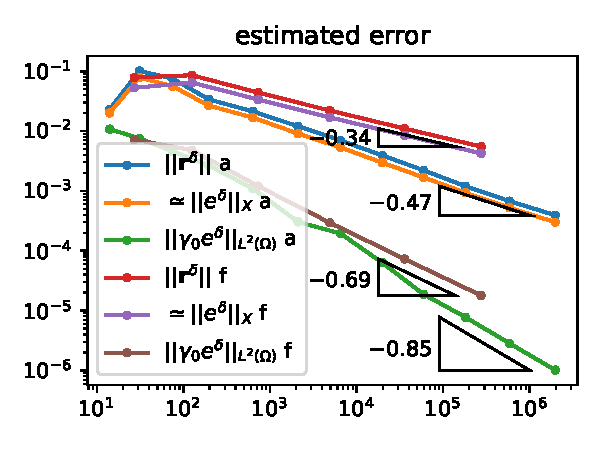
\includegraphics[width=0.5\linewidth]{smooth_adaptive_errors}
  \caption{Error progressions for the smooth problem of residual norm (solid line),
  estimated $X$-norm error (dashed), and $t=0$ time-slice error (dotted) as a function
  of $\dim X^\delta$ for adaptive (black), sparse grid (red), and full grid refinement (orange).}
  \label{fig:smooth}
\end{figure}

\subsection{Cylinder solution}
Selecting the L-shaped domain $\Omega := [-1,1]^2 \setminus [0,1]^2$ with data
$u_0 \equiv 0$ and $g(x,y) := \bbone_{{x^2 + y^2 \leq 1/4}}(x,y)$, the true
solution is unknown in closed form but known to be singular in the re-entrant
corner.\jw{is het wel singulier? of alleen minder regulier? hier wil ik een citatie of *iets* anders}
Figure~\ref{fig:cylinder} shows the error progression for this cylinder problem.
We see that the full grid rate of $\mathcal O(N^{-1/4})$ is improved to $\mathcal O(N^{-1/2}$
for adaptive refinement, recovering the rate of the smooth case.

\begin{itemize}
  \item Misschien de spatial meshes voor wat verschillende $\lambda$, of sowieso
    tellen hoeveel $\lambda$'s er zijn in dit geval? lijkt veel op de numres van FK19
\end{itemize}
\begin{figure}
  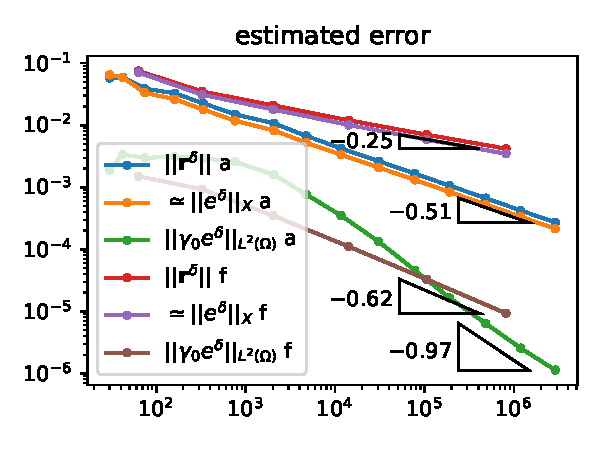
\includegraphics[width=0.5\linewidth]{cylinder_adaptive_errors}
  \caption{Error progressions for the cylinder problem of residual norm (solid line),
  estimated $X$-norm error (dashed), and $t=0$ time-slice error (dotted) as a function
  of $\dim X^\delta$ for adaptive (black), sparse grid (red), and full grid refinement (orange).}
  \label{fig:cylinder}
\end{figure}

\subsection{Second singular solution}
Selecting the unit-square domain $\Omega := [0,1]^2$ with data $u_0 := \bbone$
and $g \equiv 0$, we see the error progressions plotted in Figure~\ref{fig:singular-error}.
For the uniform refinement, we see the abhorrent convergence rate of $\O(N^{-1/11})$.
Luckily, the adaptive rate is much better at $\O(N^{-1/3})$. It is unknown
if this rate is optimal.

Figure~\ref{fig:singular-time-memory} shows the peak memory consumption in kilobytes
over $\# \dim X^\delta$ and computation time of a single application of $S^{\udelta \delta}$.
We see that the memory consumption is asymptotically linear in the number of
unknowns, whereas for the time per apply, we observe a rate of $1.04$.\jw{dit is natuurlijk groter dan 1. Is het wel acceptabel?}

\begin{figure}
  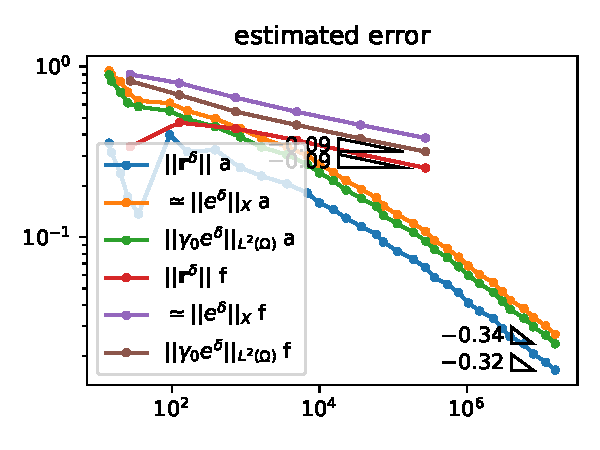
\includegraphics[width=0.5\linewidth]{singular_adaptive_errors}
  \caption{Error progression of $e^\delta := u - u^{\underline{\delta}\delta}$ for the singular problem as
  a function of $\dim X^\delta$ for adaptive and full grid refinement.\jw{excuse the terrible graph}}
  \label{fig:singular-error}
\end{figure}
\begin{figure}
  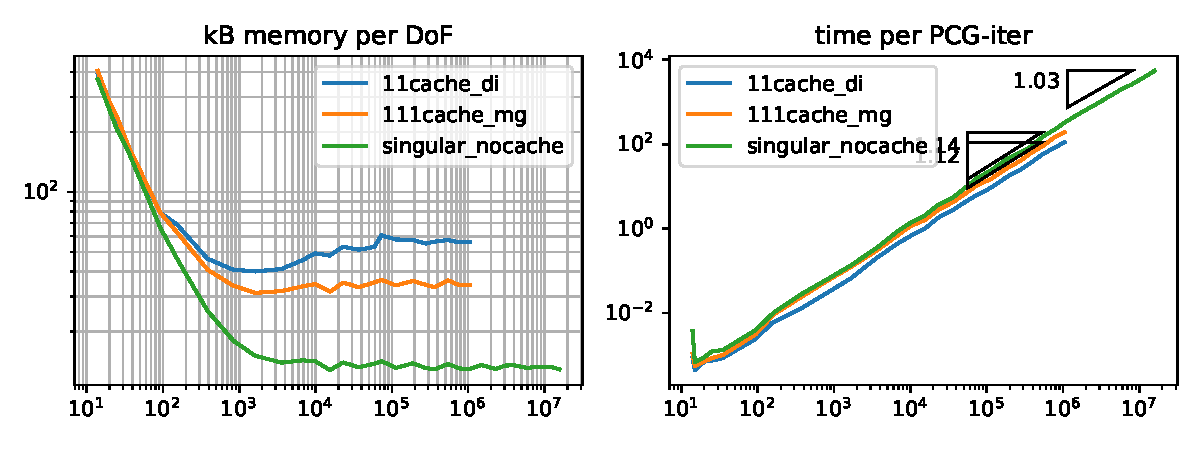
\includegraphics[width=\linewidth]{singular_mem_time.pdf}
  \caption{Time and memory progression for the singular problem for adaptive refinement.\jw{excuse the terrible graph}}
  \label{fig:singular-time-memory}
\end{figure}



\bibliography{library}
\bibliographystyle{siam}

\end{document}
